In this lecture, we will consider the problem of differentiating the \emph{solution} of ordinary differential equations (ODEs) with respect to parameters that appear in the equations and/or initial conditions.  This is as important topic in a surprising number of practical applications, such as evaluating the effect of uncertainties, fitting experimental data, or machine learning (which is increasingly combining ODE models with neural networks).  As in previous lectures, we will find that there are crucial practical distinctions between ``forward'' and ``reverse'' (``adjoint'') techniques for computing these derivatives, depending upon the number of parameters and desired outputs.

Although a basic familiarity with the concept of an ODE will be helpful to readers of this lecture, we will begin with a short review in order to establish our notation and terminology.

The video lecture on this topic for IAP 2023 was given by Dr. Frank Sch\"afer (MIT).  These notes follow the same basic approach, but differ in some minor notational details.

\subsection{Ordinary differential equations (ODEs)}
An \textbf{ordinary differential equation} (\textbf{ODE}) is an equation
for a function $u(t)$ of ``time''\footnote{Of course, the independent variable need not be time, it just needs to be a real scalar.  But in a generic context it is convenient to imagine ODE solutions as evolving in time.} $t\in\mathbb{R}$ in terms of
one or more derivatives, most commonly in the \textbf{first-order}
form 
\[
\frac{du}{dt}=f(u,t)
\]
for some right-hand-side function $f$. Note that $u(t)$ need not
be a scalar function---it could be a column vector $u\in\mathbb{R}^{n}$,
a matrix, or any other differentiable object. One could also write
ODEs in terms of higher derivatives $d^{2}u/dt^{2}$ and so on, but
it turns out that one can write any ODE in terms of first derivatives
alone, simply by making $u$ a vector with more components.\footnote{For example, the second-order ODE $\frac{d^{2}v}{dt^{2}}+\frac{dv}{dt}=h(v,t)$
could be re-written in first-order form by defining $u=\left(\begin{array}{c}
u_{1}\\
u_{2}
\end{array}\right)=\left(\begin{array}{c}
v\\
dv/dt
\end{array}\right)$, in which case $du/dt=f(u,t)$ where $f=\left(\begin{array}{c}
u_{2}\\
h(u_{1},t)-u_{2}
\end{array}\right)$. } To uniquely determine a solution of a first-order ODE, we need some
additional information, typically an \textbf{initial value} $u(0)=u_{0}$
(the value of $u$ at $t=0$), in which case it is called an \textbf{initial-value
problem}. These facts, and many other properties of ODEs, are reviewed
in detail by many textbooks on differential equations, as well as
in classes like 18.03 at MIT.

ODEs are important for a huge variety of applications, because the
behavior of many realistic systems is defined in terms of rates of
change (derivatives). For example, you may recall Newton's laws of
mechanics, in which acceleration (the derivative of velocity) is related
to force (which may be a function of time, position, and/or velocity),
and the solution $u=[\text{position},\text{velocity}]$ of the corresponding
ODE tells us the trajectory of the system. In chemistry, $u$ might
represent the concentrations of one or more reactant molecules, with
the right-hand side $f$ providing reaction rates. In finance, there
are ODE-like models of stock or option prices. \emph{Partial} differential
equations (PDEs) are more complicated versions of the same idea, for
example in which $u(x,t)$ is a function of space $x$ as well as
time $t$ and one has $\frac{\partial u}{\partial t}=f(u,x,t)$ in which $f$ may involve some spatial derivatives of $u$. 

In linear algebra (e.g.~18.06 at MIT), we often consider initial-value
problems for \emph{linear} ODEs of the form $du/dt=Au$ where $u$ is a column
vector and $A$ is a square matrix; if $A$ is a constant matrix (independent
of $t$ or $u$), then the solution $u(t)=e^{At}u(0)$ can be described in terms of a matrix exponential $e^{At}$.
More generally, there are many tricks to find explicit solutions of
various sorts of ODEs (various functions $f$). However, just as one
cannot find explicit formulas for the integrals of most functions,
there is no explicit formula for the solution of \emph{most} ODEs,
and in many practical applications one must resort to approximate
numerical solutions. Fortunately, if you supply a computer program
that can compute $f(u,t)$, there are mature and sophisticated software
libraries\footnote{For a modern and full-featured example, see the DifferentialEquations.jl
suite of ODE solvers in the Julia language.} which can compute $u(t)$ from $u(0)$ for any desired set of times
$t$, to any desired level of accuracy (for example, to 8 significant
digits).

For example, the most basic numerical ODE method computes the solution
at a sequence of times $t_{n}=n\Delta t$ for $n=0,1,2,\ldots$ simply
by approximating $\frac{du}{dt}=f(u,t)$ using the finite difference
$\frac{u(t_{n+1})-u(t_{n})}{\Delta t}\approx f(u(t_{n}),t_{n})$,
giving us the ``explicit'' timestep algorithm:
\[
u(t_{n+1})\approx u(t_{n})+\Delta t\,f(u(t_{n}),t_{n}).
\]
Using this technique, known as ``Euler's method,'' we can march
the solution forward in time: starting from our initial condition
$u_{0}$, we compute $u(t_1) = u(\Delta t)$, then $u(t_2) = u(2\Delta t)$ from $u(\Delta t)$, and so
forth. Of course, this might be rather inaccurate unless we make $\Delta t$
very small, necessitating many timesteps to reach a given time $t$,
and there can arise other subtleties like ``instabilities'' where the
error may accumulate exponentially rapidly with each timestep. It turns
out that Euler's method is mostly obsolete: there are much more sophisticated algorithms that robustly produce accurate solutions with far less
computational cost. However, they all resemble Euler's method in the
conceptual sense: they use evaluations of $f$ and $u$ at a few nearby
times $t$ to ``extrapolate'' $u$ at a subsequent time somehow, and
thus march the solution forwards through time.

Relying on a computer to obtain numerical solutions to ODEs is practically essential, but it can also make ODEs a lot more fun to work with.  If you ever took a class on ODEs, you may remember a lot of tedious labor (tricky integrals, polynomial roots, systems of equations, integrating factors, etc.) to obtain solutions by hand.  Instead, we can focus here on simply setting up the correct ODEs and integrals and trust the computer to do the rest.

\subsection{Sensitivity analysis of ODE solutions}
\label{sec:ODE-sensitivity}

\begin{figure}
    \centering
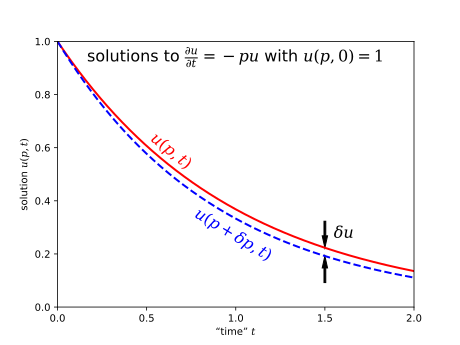
\includegraphics[width=0.6\textwidth]{figures/ode-fig.pdf}
    \caption{If we have an ordinary differential equation (ODE) $\frac{\partial u}{\partial t} = f(u, p, t)$ whose solution $u(p, t)$ depends on parameters $p$, we would like to know the change $d u = u(p + d p, t) - u(p, t)$ in the solution due to changes in $p$.  Here, we show a simple example $\frac{\partial u}{\partial t} = -pu$, whose solution $u(p,t) = e^{-p t} u(p,0)$ is known analytically, and show the change $\delta u$ from changing $p=1$ to by $\delta p = 0.1$.}
    \label{fig:ode}
\end{figure}

Often, ODEs depend on some additional parameters $p\in\mathbb{R}^{N}$
(or some other vector space). For example, these might be reaction-rate
coefficients in a chemistry problem, the masses of particles in a
mechanics problem, the entries of the matrix $A$ in a linear ODE,
and so on. So, you really have a problem of the form
\[
\frac{\partial u}{\partial t}=f(u,p,t),
\]
where the solution $u(p,t)$ depends both on time $t$ and the parameters
$p$, and in which the initial condition $u(p,0)=u_{0}(p)$ may also
depend on the parameters.

The question is, how can we compute the derivative $\partial u/\partial p$
of the solution with respect to the parameters of the ODE? By this,
as usual, we mean the linear operator that gives the first-order change
in $u$ for a change in $p$, as depicted in Fig.~\ref{fig:ode}:
\[
u(p+dp,t)-u(p,t)=\frac{\partial u}{\partial p}[dp] \qquad \mbox{(an }n\mbox{-component infinitesimal vector)},
\]
where of course $\partial u/\partial p$ (which can be thought of as an $n \times N$ Jacobian matrix) depends on $p$ and $t$.
This kind of question is commonplace. For example, it is important
in:
\begin{itemize}
\item Uncertainty quantification (UQ): if you have some uncertainty in the
parameters of your ODE (for example, you have a chemical reaction
in which the reaction rates are only known experimentally $\pm$ some
measurement errors), the derivative $\partial u/\partial p$ tells
you (to first order, at least) how sensitive your answer is to
each of these uncertainties.
\item Optimization and fitting: often, you want to choose the parameters
$p$ to maximize or minimize some objective (or ``loss'' in machine
learning). For example, if your ODE models some chemical reaction
with unknown reaction rates or other parameters $p$, you might want
to \emph{fit }the parameters $p$ to minimize the difference between
$u(p,t)$ and some experimentally observed concentrations.
\end{itemize}
In the latter case of optimization, you have a \textbf{scalar objective
function} of the solution, since to minimize or maximize something
you need a real number (and $u$ might be a vector). For example,
this could take on one of the following two forms:
\begin{enumerate}
\item A real-valued function $g(u(p,T),T) \in \mathbb{R}$ that depends on the solution $u(p,T)$ at
a particular time $T$. For example, if you have an experimental solution
$u_{*}(t)$ that you are are trying to match at $t=T$, you might
minimize $g(u(p,T),T)=\Vert u(p,T)-u_{*}(T)\Vert^{2}$. 
\item A real-valued function $G(p)=\int_{0}^{T}g(u(p,t),t)dt$ that depends on an average (here scaled by $T$)
over many times $t\in(0,T)$ of our time-dependent $g$. In the example
of fitting experimental data $u_{*}(t)$, minimizing $G(p)=\int_{0}^{T}\Vert u(p,t)-u_{*}(t)\Vert^{2}dt$
corresponds to a least-square fit to minimize the error averaged over
a time $T$ (e.g.~the duration of your experiment).
\end{enumerate}

More generally, you can give more weight to certain times than others
by including a non-negative weight function $w(t)$ in the integral:
$$G_w(p)=\int_0^\infty \underbrace{\|u(p,t)-u_*(t)\|^2}_{g(u(p,t),t)}  \, w(t) \, dt , .$$
The two cases above are simply the choices $w(t) = \delta(t-T)$ (a Dirac delta function) and $w(t) = \begin{cases} 1 & t \le T \\ 0 & \text{otherwise} \end{cases}$ (a~step function), respectively.
As discussed in Problem~\ref{prob:discrete-data}, you can let $w(t)$ be a sum of delta functions to represent data at a sequence of discrete times.

In both cases, since these are scalar-valued functions, for optimization/fitting
one would like to know the gradient $\nabla_{p}g$ or $\nabla_{p}G$,
such that, as usual,  
\[
g(u(p+dp,t),t)-g(u(p,t),t)=\left(\nabla_{p}g\right)^{T}dp
\]
so that $\pm\nabla_{p}g$ is the steepest ascent/descent direction
for maximization/minimization of $g$, respectively.
It is worth emphasizing that gradients (which we only define for scalar-valued functions) have the same shape as their inputs~$p$, so 
$\nabla_p g $ is a vector of length
$N$ (the number of parameters)  that depends on $p$ and $t$.

These are ``just derivatives,'' but probably you can see the difficulty:
if we don't have a formula (explicit solution) for $u(p,t)$, only
some numerical software that can crank out numbers for $u(p,t)$ given
any parameters~$p$ and~$t$, how do we apply differentiation rules to find $\partial u/\partial p$
or $\nabla_{p}g$? Of course, we could use finite differences as in Sec.~\ref{sec:finitedifference}---just
crank through numerical solutions for $p$ and $p+\delta p$ and subtract
them---but that will be quite slow if we want to differentiate with
respect to many parameters ($N\gg1$), not to mention giving potentially
poor accuracy. In fact, people often have \emph{huge} numbers of parameters
inside an ODE that they want to differentiate. Nowadays, our right-hand-side
function $f(u,p,t)$ can even contain a \emph{neural network} (this
is called a ``neural ODE'') with thousands or millions ($N$) of
parameters $p$, and we need all $N$ of these derivatives $\nabla_{p}g$
or $\nabla_{p}G$ to minimize the ``loss'' function $g$ or $G$.
So, not only do we need to find a way to differentiate our ODE solutions
(or scalar functions thereof), but these derivatives must be obtained
\emph{efficiently}. It turns out that there are two ways to do this,
and both of them hinge on the fact that the derivative is obtained
by \emph{solving another ODE}:
\begin{itemize}
\item \textbf{Forward} mode: $\frac{\partial u}{\partial p}$ turns out
to solve \emph{another} ODE that we can integrate with the same numerical
solvers for $u$. This gives us all of the derivatives we could want,
but the drawback is that the ODE for $\frac{\partial u}{\partial p}$
is larger by a factor of $N$ than the original ODE for $u$, so it
is only practical for small $N$ (few parameters).
\item \textbf{Reverse} (``\textbf{adjoint}'') mode: for scalar objectives,
it turns out that $\nabla_{p}g$ or $\nabla_{p}G$ can be computed
by solving a different ODE for an ``adjoint'' solution $v(p,t)$
of the \emph{same size} as $u$, and then computing some simple integrals
involving $u$ (the ``forward'' solution) and $v$.
This has the advantage of giving us all $N$ derivatives with only
about \emph{twice} the cost of solving for $u$, regardless of the
number $N$ of parameters. The disadvantage is that, since it turns
out that $v$ must be integrated ``backwards'' in time (starting
from an ``initial'' condition at $t=T$ and working back to $t=0$)
and depends on $u$, it is necessary to store $u(p,t)$ for all $t\in[0,T]$
(rather than marching $u$ forwards in time and discarding values
from previous times when they are no longer needed), which can require
a vast amount of computer memory for large ODE systems integrated
over long times.
\end{itemize}
We will now consider each of these approaches in more detail.

\subsubsection{Forward sensitivity analysis of ODEs}

Let us start with our ODE $\frac{\partial u}{\partial t}=f(u,p,t)$,
and consider what happens to $u$ for a small change $dp$ in $p$:
\begin{align*}
d\underbrace{\left(\frac{\partial u}{\partial t}\right)}_{=f(u,p,t)} &= \frac{\partial}{\partial t} (du)
=
\frac{\partial}{\partial t}
\left( \frac{\partial u}{\partial p} [ dp ]\right)=\frac{\partial}{\partial t}\left(\frac{\partial u}{\partial p}\right)[dp] \\
&=d(f(u,p,t)) = \left(\frac{\partial f}{\partial u}\frac{\partial u}{\partial p}+\frac{\partial f}{\partial p}\right)[dp],
\end{align*}
where we have used the familiar rule (from multivariable calculus)
of interchanging the order of partial derivatives---a property that
we will re-derive explicitly for our generalized linear-operator derivatives
in our lecture on Hessians and second derivatives. Equating the right-hand sides of the two lines, we see that we
have an ODE 
\[
\boxed{\frac{\partial}{\partial t}\left(\frac{\partial u}{\partial p}\right)=\frac{\partial f}{\partial u}\frac{\partial u}{\partial p}+\frac{\partial f}{\partial p}}
\]
for the derivative $\frac{\partial u}{\partial p}$, whose initial
condition is obtained simply by differentiating the initial condition
$u(p,0)=u_{0}(p)$ for $u$:
\[
\left.\frac{\partial u}{\partial p}\right|_{t=0}=\frac{\partial u_{0}}{\partial p}.
\]
We can therefore plug this into any ODE solver technique (usually
numerical methods, unless we are extremely lucky and can solve this
ODE analytically for a particular $f$) to find $\frac{\partial u}{\partial p}$
at any desired time $t$. Simple, right?

The only thing that might seem a little weird here is the \emph{shape}
of the solution: $\frac{\partial u}{\partial p}$ is a linear operator,
but how can the solution of an ODE be a linear operator? It turns
out that there is nothing wrong with this, but it is helpful to think
about a few examples:
\begin{itemize}
\item If $u,p\in\mathbb{R}$ are scalars (that is, we have a single scalar
ODE with a single scalar parameter), then $\frac{\partial u}{\partial p}$
is just a (time-dependent) number, and our ODE for $\frac{\partial u}{\partial p}$
is an ordinary scalar ODE with an ordinary scalar initial condition.
\item If $u\in\mathbb{R}^{n}$ (a ``system'' of $n$ ODEs) and $p\in\mathbb{R}$
is a scalar, then $\frac{\partial u}{\partial p}\in\mathbb{R}^{n}$
is another column vector and our ODE for $\frac{\partial u}{\partial p}$
is another system of $n$ ODEs. So, we solve two ODEs of the same
size $n$ to obtain $u$ and $\frac{\partial u}{\partial p}$.
\item If $u\in\mathbb{R}^{n}$ (a ``system'' of $n$ ODEs) and $p\in\mathbb{R}^{N}$
is a vector of $N$ parameters, then $\frac{\partial u}{\partial p}\in\mathbb{R}^{n\times N}$
is an $n\times N$ Jacobian \emph{matrix. }Our ODE for $\frac{\partial u}{\partial p}$
is effectivly system of $nN$ ODEs for all the components of this matrix,
with a matrix $\frac{\partial u_{0}}{\partial p}$ of $nN$ initial
conditions! Solving this ``matrix ODE'' with numerical methods poses
no conceptual difficulty, but will generally require about $N$ times
the computational work of solving for $u$, simply because there are
$N$ times as many unknowns. This could be expensive if $N$ is large!
\end{itemize}
This reflects our general observation of forward-mode differentiation:
it is expensive when the number $N$ of ``input'' parameters being
differentiated is large. However, forward mode is straightforward
and, especially for $N\lesssim100$ or so, is often the first method
to try when differentiating ODE solutions. Given $\frac{\partial u}{\partial p}$
, one can then straightforwardly differentiate scalar objectives by
the chain rule: 
\begin{align*}
\left.\nabla_{p}g\right|_{t=T} & =\left.\underbrace{\frac{\partial u}{\partial p}^{T}}_{\text{Jacobian}^{T}}\underbrace{\frac{\partial g}{\partial u}^{T}}_{\text{vector}}\right|_{t=T},\\
\nabla_{p}G & =\int_{0}^{T}\nabla_{p}g\,dt.
\end{align*}
The left-hand side $\nabla_p G$ is gradient of a scalar function of $N$ parameters, and hence the gradient is a vector of $N$ components.  Correspondingly, the right-hand side is an integral of an $N$-component gradient $\nabla_p g$ as well, and the integral of a vector-valued function can be viewed as simply the elementwise integral (the vector of integrals of each component).

\subsubsection{Reverse/adjoint sensitivity analysis of ODEs}

For large $N\gg1$ and scalar objectives $g$ or $G$ (etc.), we can
in principle compute derivatives \emph{much} more efficiently, with
about the same cost as computing $u$, by applying a ``reverse-mode''
or ``adjoint'' approach. In other lectures, we've obtained analogous
reverse-mode methods simply by evaluating the chain rule left-to-right
(outputs-to-inputs) instead of right-to-left. Conceptually, the process
for ODEs is similar,\footnote{This ``left-to-right'' picture can be made very explicit if we imagine
discretizing the ODE into a recurrence, e.g.~via Euler's method for
an arbitrarily small $\Delta t$, as described in the MIT course notes
\emph{\href{https://math.mit.edu/~stevenj/18.336/recurrence2.pdf}{Adjoint methods and sensitivity analysis for recurrence relations}}
by S.~G.~Johnson (2011).} but algebraically the derivation is rather trickier and less direct.
The key thing is that, if possible, we want to avoid computing $\frac{\partial u}{\partial p}$
explicitly, since this could be a prohibitively large Jacobian matrix
if we have many parameters ($p$ is large), especially if we have
many equations ($u$ is large). 

In particular, let's start with our forward-mode sensitivity analysis,
and consider the derivative $G'=(\nabla_{p}G)^{T}$ where $G$ is
the integral of a time-varying objective $g(u,p,t)$ (which we allow
to depend explicitly on $p$ for generality). By the chain rule,
\[
G'=\int_{0}^{T}\left(\frac{\partial g}{\partial p}+\frac{\partial g}{\partial u}\frac{\partial u}{\partial p}\right)dt,
\]
which involves our unwanted factor $\frac{\partial u}{\partial p}$.
To get rid of this, we're going to use a ``weird trick''
\todo{I don't think this needs
to look like a weird trick, but i have
to remember why, EVEN Lagrange
multipliers don't have to be taught
as a weird trick, but I know they often are}
(much like Lagrange
multipliers) of adding \emph{zero} to this equation:
\[
G'=\int_{0}^{T}\left[\left(\frac{\partial g}{\partial p}+\frac{\partial g}{\partial u}\frac{\partial u}{\partial p}\right)+v^{T}\underbrace{\left(\frac{\partial}{\partial t}\left(\frac{\partial u}{\partial p}\right)-\frac{\partial f}{\partial u}\frac{\partial u}{\partial p}-\frac{\partial f}{\partial p}\right)}_{=0}\right]dt
\]
for some function $v(t)$ of the \emph{same shape as u} that multiplies our ``forward-mode'' equation for $\partial u/ \partial p$. (If $u\in\mathbb{R}^{n}$
then $v\in\mathbb{R}^{n}$; more generally, for other vector spaces,
read $v^{T}$ as an inner product with $v$.) The new term $v^T (\cdots)$
is zero because the parenthesized expression is precisely the ODE satisfied by $\frac{\partial u}{\partial p}$,
as obtained in our forward-mode analysis above,  \emph{regardless} of
$v(t)$. This is important because it allows us the freedom to \emph{choose}
$v(t)$ to \emph{cancel} the unwanted $\frac{\partial u}{\partial p}$
term. In particular, if we first \emph{integrate by parts} on the
$v^{T}\frac{\partial}{\partial t}\left(\frac{\partial u}{\partial p}\right)$
term to change it to $-\left(\frac{\partial v}{\partial t}\right)^{T}\frac{\partial u}{\partial p}$
plus a boundary term, then re-group the terms, we find:
\[
G'=\left.v^{T}\frac{\partial u}{\partial p}\right|_{0}^{T}+\int_{0}^{T}\left[\frac{\partial g}{\partial p}-v^{T}\frac{\partial f}{\partial p}+\underbrace{\left(\frac{\partial g}{\partial u}-v^{T}\frac{\partial f}{\partial u}-\left(\frac{\partial v}{\partial t}\right)^{T}\right)}_{\text{want to be zero!}}\frac{\partial u}{\partial p}\right]dt\:.
\]
If we could now set the $(\cdots)$ term to zero, then the unwanted
$\frac{\partial u}{\partial p}$ would vanish from the integral calculation
in $G'$. We can accomplish this by \emph{choosing} $v(t)$ (which
could be \emph{anything} up to now) to satisfy the \textbf{``adjoint''
ODE}:
\[
\boxed{\frac{\partial v}{\partial t}=\left(\frac{\partial g}{\partial u}\right)^{T} - \left(\frac{\partial f}{\partial u}\right)^{T}v}.
\]
What initial condition should we choose
for $v(t)$? Well, we can use this choice to get rid of the boundary
term we obtained above from integration by parts: 
\[
\left.v^{T}\frac{\partial u}{\partial p}\right|_{0}^{T}=v(T)^{T}\underbrace{\left.\frac{\partial u}{\partial p}\right|_{T}}_{\text{unknown}}-v(0)^{T}\underbrace{\frac{\partial u_{0}}{\partial p}}_{\text{known}}.
\]
Here, the unknown $\left.\frac{\partial u}{\partial p}\right|_{T}$
term is a problem---to compute that, we would be forced to go back
to integrating our big $\frac{\partial u}{\partial p}$ ODE from forward
mode. The other term is okay: since the initial condition $u_{0}$
is always given, we should know its dependence on $p$ explicitly
(and we will simply have $\frac{\partial u_{0}}{\partial p}=0$ in
the common case where the initial conditions don't depend on $p$).
To eliminate the $\left.\frac{\partial u}{\partial p}\right|_{T}$
term, therefore, we make the choice 
\[
\boxed{v(T)=0}.
\]
Instead of an \emph{initial} condition, our adjoint ODE has a \textbf{final
condition}. That's no problem for a numerical solver: it just means
that the \textbf{adjoint ODE is integrated }\textbf{\emph{backwards}}\textbf{
in time}, starting from $t=T$ and working down to $t=0$. Once we
have solved the adjoint ODE for $v(t)$, we can plug it into our equation
for $G'$ to obtain our gradient by a simple integral:
\[
\nabla_{p}G=\left(G'\right)^{T}=-\left(\frac{\partial u_{0}}{\partial p}\right)^{T}v(0)+\int_{0}^{T}\left[\left(\frac{\partial g}{\partial p}\right)^{T}-\left(\frac{\partial f}{\partial p}\right)^{T}v\right]dt\:.
\]
(If you want to be fancy, you can compute this $\int_{0}^{T}$ simultaneously
with $v$ itself, by augmenting the adjoint ODE with an additional
set of unknowns and equations representing the $G'$ integrand. But
that's mainly just a computational convenience and doesn't change
anything fundamental about the process.)

The only remaining annoyance is that the adjoint ODE depends on $u(p,t)$
for all $t\in[0,T]$. Normally, if we are solving the ``forward''
ODE for $u(p,t)$ numerically, we can ``march'' the solution $u$
forwards in time and only store the solution at a few of the most
recent timesteps. Since the adjoint ODE starts at $t=T$, however,
we can only start integrating $v$ after we have completed the calculation
of $u$. This requires us to save essentially \emph{all} of our previously
computed $u(p,t)$ values, so that we can evaluate $u$ at arbitrary
times $t\in[0,T]$ during the integration of $v$ (and $G'$). This
can require a lot of computer memory if $u$ is large (e.g.~it could
represent \emph{millions} of grid points from a spatially discretized
PDE, such as in a heat-diffusion problem) and many timesteps $t$
were required. To ameliorate this challenge, a variety of strategies
have been employed, typically centered around ``checkpointing''
techniques in which $u$ is only saved at a subset of times $t$,
and its value at other times is obtained during the $v$ integration
by \emph{re-computing} $u$ as needed (numerically integrating the
ODE starting at the closest ``checkpoint'' time). A detailed discussion
of such techniques lies outside the scope of these notes, however.

\subsection{Example}

Let us illustrate the above techniques with a simple example. Suppose
that we are integrating the scalar ODE 
\[
\frac{\partial u}{\partial t}=f(u,p,t)=p_{1}+p_{2}u+p_{3}u^{2}=p^{T}\left(\begin{array}{c}
1\\
u\\
u^{2}
\end{array}\right)
\]
for an initial condition $u(p,0)=u_{0}=0$ and three parameters $p \in \mathbb{R}^3$. (This is probably simple
enough to solve in closed form, but we won't bother with that here.) We will also consider the scalar function 
\[
G(p)=\int_{0}^{T}\underbrace{\left[u(p,t)-u_{*}(t)\right]^{2}}_{g(u,p,t)}dt
\]
that (for example) we may want to minimize for some given $u_{*}(t)$ (e.g.~experimental
data or some given formula like $u_{*}=t^{3}$), so we are hoping to compute $\nabla_{p}G$.

\subsubsection{Forward mode}

The Jacobian matrix $\frac{\partial u}{\partial p}=\left(\begin{array}{ccc}
\frac{\partial u}{\partial p_{1}} & \frac{\partial u}{\partial p_{2}} & \frac{\partial u}{\partial p_{3}}\end{array}\right)$ is simply a row vector, and satisfies our ``forward-mode'' ODE:
\[
\frac{\partial}{\partial t}\left(\frac{\partial u}{\partial p}\right)=\frac{\partial f}{\partial u}\frac{\partial u}{\partial p}+\frac{\partial f}{\partial p}=\left(p_{2}+2p_{3}u\right)\frac{\partial u}{\partial p}+\left(\begin{array}{ccc}
1 & u & u^{2}\end{array}\right)
\]
for the initial condition $\left.\frac{\partial u}{\partial p}\right|_{t=0}=\frac{\partial u_{0}}{\partial p}=0$.
This is an inhomogeneous system of three coupled \emph{linear} ODEs,
which might look more conventional if we simply transpose both sides:
\[
\frac{\partial}{\partial t}\underbrace{\left(\begin{array}{c}
\frac{\partial u}{\partial p_{1}}\\
\frac{\partial u}{\partial p_{2}}\\
\frac{\partial u}{\partial p_{3}}
\end{array}\right)}_{(\partial u/\partial p)^{T}}=\left(p_{2}+2p_{3}u\right)\left(\begin{array}{c}
\frac{\partial u}{\partial p_{1}}\\
\frac{\partial u}{\partial p_{2}}\\
\frac{\partial u}{\partial p_{3}}
\end{array}\right)+\left(\begin{array}{c}
1\\
u\\
u^{2}
\end{array}\right).
\]
The fact that this depends on our ``forward'' solution $u(p,t)$
makes it not so easy to solve by hand, but a computer can solve it numerically
with no difficulty.  On a computer, we would probably solve for $u$ and $\partial u/ \partial p$\emph{simultaneously} by combining the two ODEs into a single ODE with~4 components:
\[
\frac{\partial}{\partial t}\left(\begin{array}{c}
u \\
(\partial u/\partial p)^{T}
\end{array}\right) =
\left(\begin{array}{c}
p_{1}+p_{2}u+p_{3}u^{2} \\
\left(p_{2}+2p_{3}u\right) (\partial u/\partial p)^{T} +\left(\begin{array}{c}
1\\
u\\
u^{2}
\end{array}\right)
\end{array}\right).
\]
Given $\partial u/\partial p$, we can then plug this into the chain rule for
$G$:
\[
\nabla_{p}G=2\int_{0}^{T}\left[u(p,t)-u_{*}(t)\right]\frac{\partial u}{\partial p}^{T}\,dt
\]
(again, an integral that a computer could evaluate numerically).


\subsubsection{Reverse mode}

In reverse mode, we have an adjoint solution $v(t)\in\mathbb{R}$
(the same shape as $u$) which solves our adjoint equation 
\[
 \frac{\partial v}{dt}=\left(\frac{\partial g}{\partial u}\right)^{T} -\left(\frac{\partial f}{\partial u}\right)^{T}v =2\left[u(p,t)-u_{*}(t)\right] - \left(p_{2}+2p_{3}u\right)v
\]
with a \emph{final} condition $v(T)=0.$ Again, a computer can solve
this numerically without difficulty (given the numerical ``forward''
solution $u$) to find $v(t)$ for $t\in[0,T]$. Finally, our gradient
is the integrated  product:
$$
\nabla_{p}G = -\int_{0}^{T}
\left(
\begin{array}{c} 1 \\ u \\ u^{2} \end{array}
\right)
v\,dt\:.
$$

Another useful exercise is to consider a $G$ that takes the form of a summation:
\begin{problem}
\label{prob:discrete-data}
Suppose that $G(p)$ takes the form of a sum of $K$ terms:
$$
G(p) = \sum_{k=1}^{K} g_k(p,u(p,t_k))
$$
for times $t_k \in (0, T)$ and functions $g_k(p,u)$.  For example, this could arise in least-square fitting of  experimental data $u_*(t_k)$ at $K$ discrete times, with $g_k(u(p,t_k)) = \Vert u_*(t_k) -u(p,t_k)\Vert^2 $ measuring the squared difference between $u(p,t_k)$ and the measured data at time $t_k$.
\begin{enumerate}
    \item Show that such a $G(p)$ can be expressed as a special case of our formulation in this chapter, by defining our function $g(u,t)$ using a sum of Dirac delta functions $\delta(t - t_k)$.
    \item Explain how this affects the adjoint solution $v(t)$: in particular, how the introduction of delta-function terms on the right-hand side of $dv/dt$ causes $v(t)$ to have a sequence of discontinuous jumps.  (In several popular numerical ODE solvers, such discontinuities can be incorporated via discrete-time ``callbacks''.)
    \item Explain how these delta functions  may also introduce a summation into the computation of $\nabla_p G$, but only if $g_k$ depends explicitly on~$p$ (not just via~$u$).
\end{enumerate}
\end{problem}


\subsection{Further reading}

A classic reference on reverse/adjoint differentiation of ODEs (and
generalizations thereof), using notation similar to that used today
(except that the adjoint solution $v$ is denoted $\lambda(t)$, in an
homage to Lagrange multipliers), is Cao~et~al.~(2003) (\url{https://doi.org/10.1137/S1064827501380630}), and a more recent review article is Sapienza~et~al.~(2024) (\url{https://arxiv.org/abs/2406.09699}).
See also the SciMLSensitivity.jl package (\url{https://github.com/SciML/SciMLSensitivity.jl})
for sensitivity analysis with Chris Rackauckas's amazing DifferentialEquations.jl
software suite for numerical solution of ODEs in Julia. There is a
nice 2021 YouTube lecture on adjoint sensitivity of ODEs (\url{https://youtu.be/k6s2G5MZv-I}),
again using a similar notation. A discrete version of this process
arises for recurrence relations, in which case one obtains a reverse-order
``adjoint'' recurrence relation as described in MIT course notes
by S.~G.~Johnson (\url{https://math.mit.edu/~stevenj/18.336/recurrence2.pdf}).

The differentiation methods in this chapter (e.g.~for $\partial u/\partial p$ or $\nabla_p G$) are derived assuming that the ODEs are solved exactly: given the exact ODE for $u$, we derived an exact ODE for the derivative. On a computer, you will solve these forward and adjoint ODEs approximately, and in consequence the resulting derivatives will only be approximately correct (to the tolerance specified by your ODE solver).  This is known as a {\bf differentiate-then-discretize} approach, which has the advantage of simplicity (it is independent of the numerical solution scheme) at the expense of slight inaccuracy (your approximate derivative will not exactly predict the first-order change in your approximate solution $u$).   The alternative is a {\bf discretize-then-differentiate} approach, in which you first approximate (``discretize'') your ODE into a discrete-time recurrence formula, and then \emph{exactly} differentiate the recurrence.  This has the advantage of exactly differentiating your approximate solution, at the expense of complexity (the derivation is specific to your discretization scheme).  Various authors discuss these tradeoffs and their implications, e.g.~in chapter~4 of M.~D.~Gunzburger's \href{https://doi.org/10.1137/1.9780898718720.ch4}{{\it Perspectives in Flow Control and Optimization}} (2002) or in papers like \href{https://dl.acm.org/doi/10.1007/s00158-013-1024-4}{Jensen~et~al.~(2014)}.